% !TeX root = ../main.tex
\section{Các Biến Thể Nhiều Người}
\label{sec:variants}

Cùng một bộ luật cốt lõi---di chuyển bằng cú nhảy, ăn bằng kẹp lật, bảo
toàn tổng số quân---được giữ nguyên qua cả ba biến thể; chỉ kích thước
bàn, số quân mỗi phe và số phe thay đổi (Bảng~\ref{tab:board_size}). Chế
độ 4 người dùng bàn 7{\texttimes}7 cắt tám ô ở bốn góc, tạo hình gần bát
giác cân đối cho bốn hướng tiến quân (Hình~\ref{fig:multiboard}); chế độ
3 người dùng bàn 7{\texttimes}6 chỉ cắt hai góc dưới.

\begin{figure}[H]
  \centering
  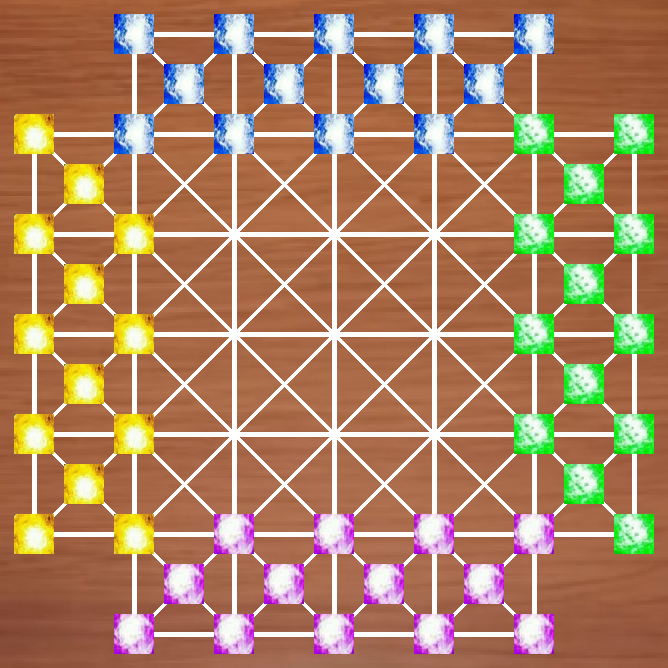
\includegraphics[width=0.52\linewidth]{figures/board_4p.png}
  \caption{Vị trí xuất phát chế độ 4 người (ảnh chụp trực tiếp từ trò
  chơi): bàn 7{\texttimes}7 cắt tám ô ở bốn góc tạo hình gần bát giác cân
  đối cho bốn hướng tiến quân; bốn phe Lam, Xanh lá, Tím, Vàng mỗi phe 13
  quân. Toạ độ và vị trí xuất phát chính xác ở
  Phụ lục~\ref{app:multistart}.}
  \label{fig:multiboard}
\end{figure}

\subsection{Chế Độ 2 Người}
Bàn cờ 5{\texttimes}5 đỉnh. Mỗi bên 14 quân (10 đỉnh + 4 tâm).
Màu: Vàng và Xanh lá. Đây là chế độ được mô hình hoá đầy đủ ở
Phụ lục~\ref{app:formal} và dùng Minimax Alpha-Beta cổ điển (Mục~\ref{sec:ai}).

\subsection{Chế Độ 3 Người}

\begin{figure}[H]
  \centering
  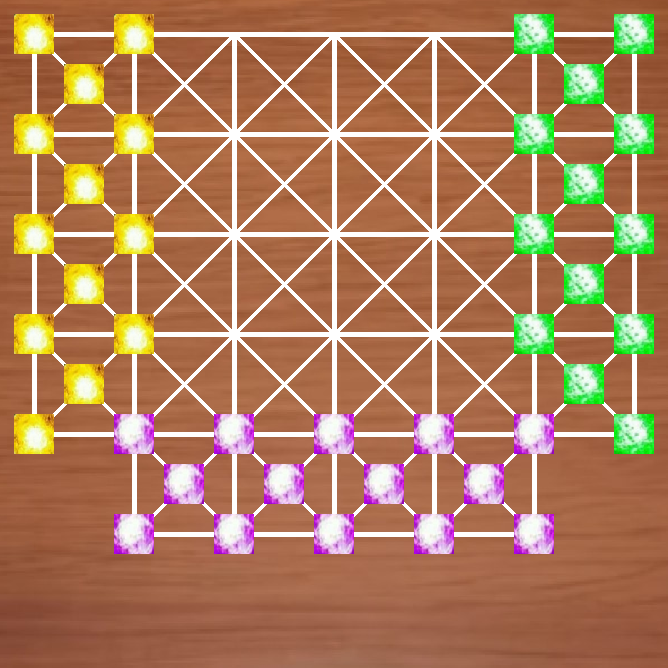
\includegraphics[width=0.52\linewidth]{figures/board_3p.png}
  \caption{Vị trí xuất phát chế độ 3 người (ảnh chụp trực tiếp từ trò
  chơi): bàn 7{\texttimes}6 cắt bốn ô ở hai góc dưới; ba phe Vàng, Xanh
  lá, Tím. Cấu hình \emph{không cân đối}---hai phe 13 quân, phe thứ ba 14
  quân (Phụ lục~\ref{app:multistart}).}
  \label{fig:board3p}
\end{figure}

Bàn cờ 7{\texttimes}6 với 4 ô ở hai góc dưới bị loại.
Hai phe có 13 quân và phe thứ ba có 14 quân (cấu hình chính xác và lưu ý
bất đối xứng ở Phụ lục~\ref{app:multistart}). Màu: Vàng, Xanh lá, Tím.
Chế độ này giới thiệu
\emph{động lực liên minh}: người chơi phải cân nhắc không chỉ tấn công
đối thủ trực tiếp mà còn tránh tạo lợi thế cho đối thủ thứ ba. Vì điểm
số không còn đối nghịch hoàn toàn giữa hai phe, AI chuyển sang Paranoid
Minimax (Mục~\ref{sec:ai})---giả định bi quan rằng hai đối thủ còn lại
phối hợp chống mình.

\subsection{Chế Độ 4 Người}
Bàn 7{\texttimes}7 cắt 8 ô ở bốn góc, mỗi bên 13 quân.
Màu: Lam, Xanh lá, Tím, Vàng. Như ở chế độ 3 người, mỗi người chơi phải
tính đến cả ba đối thủ cùng lúc.
